% Metódy inžinierskej práce

\documentclass[10pt,slovak,a4paper]{article} 

\usepackage[slovak]{babel}
%\usepackage[T1]{fontenc}
\usepackage[IL2]{fontenc} % lepšia sadzba písmena Ľ než v T1
\usepackage[utf8]{inputenc}
\usepackage{graphicx}
\usepackage{url} % príkaz \url na formátovanie URL
\usepackage{hyperref} % odkazy v texte budú aktívne (pri niektorých triedach dokumentov spôsobuje posun textu)
\usepackage{amsmath}

\graphicspath{{./images/}}
\usepackage{cite}
\usepackage{pgfplots}
\pgfplotsset{width=10cm,compat=1.9}


\pagestyle{headings}

\title{Ako vyhľadávajú Google Maps\thanks{Semestrálny projekt v predmete Metódy inžinierskej práce, ak. rok 2023/24, vedenie: Vladimír Mlynarovič}} % meno a priezvisko vyučujúceho na cvičeniach

\author{Adrián Maslák\\[2pt]
	{\small Slovenská technická univerzita v Bratislave}\\
	{\small Fakulta informatiky a informačných technológií}\\
	{\small \texttt{xmaslaka@stuba.sk}}
	}

\date{\small 16. December 2023} % upravte



\begin{document}

\maketitle

\begin{abstract}
Google Maps je sofistikovaný systém máp priamo v naších zariadeniach ktorý nám umožňuje nájsť nové miesta, získať pokyny na prepravu z bodu A do bodu B. Pomôcka ktorú každodenne používa viac než miliarda používateľov.
	Aplikácia Google Maps je písaná v jazykoch C++, JavaScript, XML a AJAX.  Na vypočítanie najkratšej trasy sú použíté dva algoritmy, Dijkstrov algoritmus a A* algoritmus ktoré sú najrýchlejšie a najefektívnejšie pri hľadaní najkratšej trasy v grafoch, kde si môžeme cesty predstaviť ako jeden graf. Do týchto vyhľadavaní zasahujú aj reálne faktory ako hustota premávky alebo počasie. Vďaka dlhému vývoju nám táto aplikácia umožnuje nájsť aj alternatívne trasy a všetky dopravné obmedzenia.
	Článok končí objasnením fungovania tohto komplexného systémum, spresnením využitých funkcií a algoritmov.

Témou tohto článku je vyhľadávanie Google Maps. Google maps je každodenná pomôcka miliónov používateľov a preto treba objasniť ako to celé vlastne funguje. Pod pojmom fungovania máme na mysli systém vďaka ktorému môžeme využívať náš prenosný atlas, ktorý nás dostane z bodu A do bodu B. Celkovo sa článok zameriáva na vyhľadávacie algoritmy ale aj na vplyv premávky a udalostí v reálnom čase na vyhľadanie najkratšej, najrýchlejšej a najefektívnejšej trasy. Z pohľadu laika možno sa to zdá ako zanedbateľná vec, ale pre obecenstvo s technickým zameraním to je komplexné riešenie ktoré zahrňuje enormné množstvo úsila, pozornosti a logického myslenia. 
\end{abstract}



\section{Úvod}
\cite{GOOGLEMAPS}
Google Mapy sú jednou z najvačších inovácií v histórií technológie. \cite{GMaps}


Príchod tejto aplikácie od giganta v technologickom svete Google Inc. Google Mapy umožňujú používateľom hľadať najkratšie a najefektívnejšie trasy do ich destinácie. Google Mapy získali takmer 70 miliónov používateľov.\cite{GmapWorks} Postupom času boli pridané mnohé funkcie okrem navigácie. Technológia a algoritmy použité v tomto systéme sú veľmi pokročilé. \cite{behindGmap}Google uchovávava a analyzuje nespočetné množstvo dát vrátane historických údajov a údajov ktoré prebiehajú v reálnom čase, to je čo robí Google Mapy neskutočne progresívne a presné.

\section{Google Maps: Použité algoritmy}
Google Maps, ako jedna z najpopulárnejších a najpoužívanejších navigačných aplikácií na svete, poskytuje užívateľom detailné mapy, presné navigačné pokyny a cenné dopravné informácie. Za týmto úspechom stojí široké spektrum sofistikovaných algoritmov a technológií, ktoré pracujú v pozadí, aby zabezpečili, že každá cesta je čo najefektívnejšia a najbezpečnejšia.
\cite{Algoritmy} Tieto algoritmy sú základom Google Maps a umožňujú aplikácii riešiť rôzne výzvy, ako sú plánovanie trás, predpovedanie a riadenie dopravy, ako aj rýchla adaptácia na meniace sa podmienky v reálnom čase. Vďaka pokročilým výpočtovým metódam a masívnemu využitiu dát Google Maps dokáže efektívne spracovávať a analyzovať obrovské množstvo informácií, čo z neho robí mimoriadne presný a užívateľsky prívetivý nástroj.
\subsection{Dijkstrov algoritmus}
Je to veľmi efektívny algoritmus vynájdený Edsger W. Dijkstrom v roku 1956. \cite{Djikstra's} Tento algoritmus sa používa pri hľadaní najkratšej trasy medzi bodmi v ohodnotených grafoch. Komplexnosť riešení tohto grafu vieme vyjdariť ako $\boldsymbol{\theta((V + E) \log V)}$

\begin{figure} [h]
 \centering
 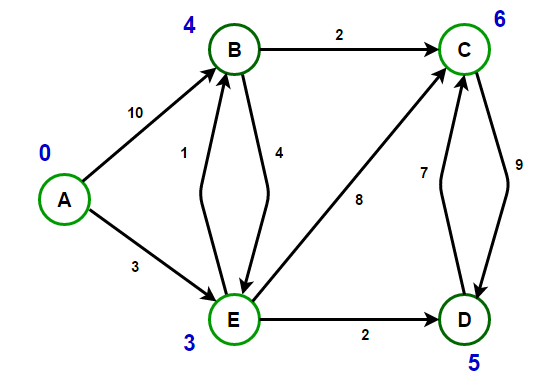
\includegraphics[width=6cm]{dijkstra}
\caption{Dijkstrov Algoritmus}

\end{figure}

Google Mapy zapájajú grafové dátové štruktúry na výpočet najkratšej trasy zo zdroja (bod A) do cieľovej destinácie (bod B). Grafová analýza obsahuje mnoho bodov a hrán cez ktoré tento algoritmus putuje a nachádza najkratšiu trasu. Aj keď je tento algoritmus jeden z najpopulárnejších, enormné množstvo bodov a hrán môže zapríčiniť zlyhanie v dôsledku predĺženia času alebo nedostatku pamäte. Drastické zväčšovanie grafu limituje efektivitu algoritmu.
\cite{Algoritmy2}
\textbf{Dijkstrov algoritmus} je základom teórie grafov, bol kľúčovým bodom na vývoj digitálnych navigačných systémov. Zatiaľ čo aktuálne algoritmy používané Google maps sú omnoho viac komplexnejšie. Dijkstrovo dedičstvo vo vyhľadávaní najkratšej trasy je stále nepopierateľné. Je to klasický prípad ako teoretické koncepty počítačových vied prenikajú do praktického sveta s obrovským vplyvom na naše životy.

\subsection{A* algoritmus}\label{Astar}
A* Algogoritmus je flexibilný, viac efektívny. Tento algoritmus patrí do skupiny heuristických \ref{heuristika} algoritmov.
Google Mapy ho momentálne používajú na hľadanie najkratšej trasy. Dokáže prijať väčšie grafy, čo je výhoda oproti Dijkstrovmu algoritmu. A* algoritmus je široko používaný algoritmus, keďže používa a kombinuje informácie z iných algoritmov. Vzhľadom na to, že A* poskytuje rýchle a optimalizované riešenia, je ideálny pre real-time aplikácie ako Google Maps, kde užívatelia očakávajú rýchle a presné navigačné pokyny. Komplexnosť riešení tohto grafu vieme vyjadriť ako $\boldsymbol{ \theta(b^d) }$
\paragraph{}


\begin{figure}[h]
  \centering
  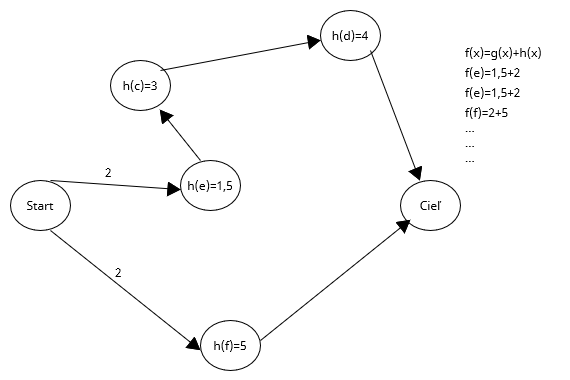
\includegraphics[width=8cm]{a-star}
  \caption{A* Algoritmus}
\end{figure}
	\begin{enumerate}
\item Inicializácia
	\begin{itemize}
\item
Algoritmus začína s otvoreným zoznamom, kde je začiatočný uzol a s prázdny zatvoreným zoznamom.
\end{itemize}
\item  Výber hrany
	\begin{itemize}
	\item Algoritmus vyberie uzol z otvoreného zoznamu s najnižšou hodnotou $$ f(x)=g(x)+h(x)$$
	\item g(x) :- Cena cesty od štartovacieho bodu k danému uzlu a 
	\item h(x):- Odhadovaná hodnota do cieľa z bodu n. - Heuristická časť algoritmu.
	\item f(x):- Celková vyčíslená hodnota každého bodu.
	\end{itemize}
\item Opakovanie
	\begin{itemize}
	\item Pre každého suseda vybraného uzla sa vypočíta hodnota f(x) a ak nie je v otvorenom zozname, pridá sa do neho.	
	\item  Tento proces sa opakuje, kým algoritmus nenájde cieľový uzol alebo kým otvorený zoznam neostane prázdny (čo znamená, že cesta neexistuje).
	\end{itemize}
\item Výstup
	\begin{itemize}
	\item Keď sa dosiahne cieľový uzol, algoritmus rekonštruuje cestu od cieľa späť k počiatočnému bodu (cesta sa obvykle ukladá prostredníctvom odkazov na rodičovské uzly).
Výsledkom je najkratšia odhadovaná trasa.
	\end{itemize}
\end{enumerate}
Celková váha vypočítaná algoritmom by nemala byť preceňovaná, keďže ide o heuristický algoritmus. Teda váha grafu, cesta po hranách z bodu A do bodu B má byť rovnaká alebo vačšia ako odhad váhy grafu. Narozdiel od iných algoritmov sa tento zaoberá priamo na cieľovú destináciu (bod B). Zvyšné body a hrany neberie do úvahy. Taktiež berie do úvahy parametre ako časové požiadavky, vzdialenosť, optimalizáciu a vyberanie lepšej trasy. 
\subsection{Porovnanie}
V súčasnej dobe sa pri vývoji aplikácií ako Google Maps čoraz viac kládne dôraz na efektívnosť a presnosť pri hľadaní trás. Dve základné techniky, ktoré sa pri tom používajú, sú Dijkstrov algoritmus a A* algoritmus. Každý z týchto algoritmov má svoje špecifické vlastnosti a použitie, ktoré ich robia vhodnými pre rôzne druhy úloh v rámci navigačných systémov. Dijkstrov algoritmus je známy pre jeho presnosť a jednoduchosť, zatiaľ čo A* algoritmus vyniká svojou efektívnosťou v komplexných a rozsiahlych grafoch vďaka použitiu heuristických metód.
\begin{table}[h]
\centering
\begin{tabular}{|l|l|l|}
\hline
\textbf{Faktor} & \textbf{Dijkstrov Algoritmus} & \textbf{A* Algoritmus} \\
\hline
Funkcia & Najkratšia trasa & Odhad najkratšej trasy \\
\hline
Zložitosť & O((V + E) log V) & O(b^d) \\
\hline
Použitie& Malé grafy & Veľké grafy \\
\hline
Nevýhody & Komplexné grafy & Závislý od heuristiky \\
\hline
 Google Maps & Tradičné plánovanie ciest & Dynamické plánovanie ciest \\
\hline
\end{tabular}
\caption{Porovnanie Dijkstrovho algoritmu a A* algoritmu}
\label{table:comparison}
\end{table}




\section{Street View}\label{Street}
V roku 2007, \cite{StreeView} Google maps predstavilo novú funkciu s názvom Street View. Táto neskutočná inovácia sa osvedčila ako obrovský milník v histórií navigácie a GPS. Street View poskytuje 3-rozmerný, HD, panoramatický pohľad na dokumentované ulice, mestá, cesty a mnohé ďalšie oblasti priamo z vášho mobilného telefónu alebo počítača. Prekvapivo tieto záznamy sú manuálne vyhotovené tímom Google Maps pomocou auta vybaveným viackamerovou sústavou a ďalším potrebným vybavením. Tieto záznamy sú následné použité na generovanie street view.
\begin{figure}
\centering
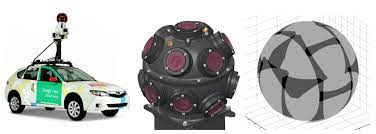
\includegraphics[width=10cm]{streetview.jpg}
\caption{Street View vybavenie}

\end{figure}



Následne prichádza proces spájania týchto fotografií. Tieto fotografie sú snímané v panoramatickom režime ktorý dokáže zachytiť širší uhol scenérie. Na spojenie fotografií tím Google Maps vytvoril nový algoritmus na základe optického toku, ktorého princípom je jemne deformovať každú z fotiek tak, aby sa medzi sebou prekrývali. Tento proces musí byť kontrolovaný a opakovaný niekoľko krát, aby nevznikali vizuálne anomálie. Na zjednodušenie procesu spájania fotografií ho môžeme rozdeliť na dva menšie kroky:
\begin{enumerate}
\item Optický tok
\begin{itemize}
\item Prvý krok je nájsť korešpondujúce pixely a ich lokáciu kde sa prekrývajú. Použitím algoritmov neskôr vypočítame optický tok z jedného obrázka na druhý. Toto poskytuje jemné a husté korespondenčné pole.
\begin{figure}[h]
\centering
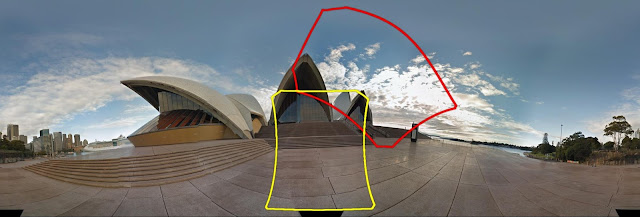
\includegraphics[width=8cm]{opticalflow.jpg}
\caption{Optický tok}
\end{figure}


\end{itemize}
\item Globálna optimalizácia
\begin{itemize}
\item
Druhý krok je deformovať obrázky tak, aby sa súčasne zarovnávali s korešpondečnými bodmi z prekrývajúcich sa regiónov. Keď sú spájané do jednej veľkej panorámy, súprava deformovaných obrázkov by mala byť spojená korektne. 
\begin{figure}[h]
\centering
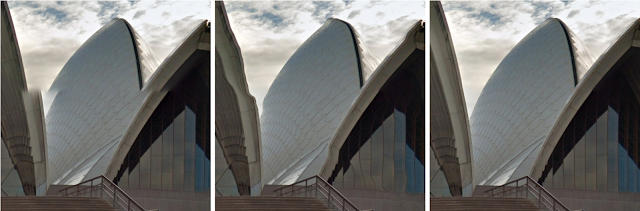
\includegraphics[width=8cm]{globaloptimalization.png}
\caption{Spajanie panorámy}
\end{figure}

\end{itemize}
\end{enumerate}
\section{Porovnanie pokrytia}
Funkcia Street View funguje už od spomínaného roku 2007, po spustení sa masívne rozrástla na obrovský projekt mapovania zemegule.  Avšak, miera pokrytia Street View sa líši v rôznych regiónoch sveta, čo je ovplyvnené rôznymi faktormi, vrátane geografie, infraštruktúry a priorit spoločnosti Google. V nasledujúcom grafu porovnávame odhadované percentuálne pokrytie Street View na štyroch hlavných kontinentoch: Amerika, Európa, Ázia a Afrika. Toto porovnanie nám poskytuje prehľad o rozsahu a dosahu tohto technologického úsilia a ukazuje, ako digitálna dostupnosť a mapovanie majú nerovnomerné rozloženie na celom svete. Dôležité je poznamenať, že tieto údaje sú približné a môžu sa líšiť od aktuálnych podmienok.\cite{coverage}

\begin{tikzpicture}
\begin{axis}[
    ybar,
    enlargelimits=0.15,
    legend style={at={(0.5,-0.15)},
      anchor=north,legend columns=-1},
    ylabel={Pokrytie v \%},
    symbolic x coords={Amerika, Európa, Ázia, Afrika},
    xtick=data,
    nodes near coords,
    nodes near coords align={vertical},
    ymin=0,ymax=100
]
\addplot coordinates {(Amerika,85) (Európa,70) (Ázia,69) (Afrika,28)};
\legend{Pokrytie Street View}
\end{axis}
\end{tikzpicture}




\section{Analýza cestnej premávky} \label{Analyza}
Google Mapy narozdiel od iných GPS a navigačných systémov používajú aktuálne dáta. \cite{AI-and-traffic}Čo umožnuje vyberať rýchlejšie trasy, vyhnúť sa dopravným obmedzeniam. 
Google Mapy analyzujú cestnú premávku kombinácou aktuálnych dát od používateľov a historických vzorov dopravnej situácie. Machine learning techniky ako grafové neurónové siete tieto predpovede spresňujú. Google Mapy taktiež zvažujú použitie smerodajných údajov od miestnych samospráv za účelom zlepšiť predpovede na základe dopravných podmienok ako stav cesty, maximálna povolená rýchlosť alebo nehodovosť určitých úsekov. Tieto rôznorodé dáta umožňujú odporúčiť najefektívnejšiu cestu ako aj predpovedať dopravné podmienky.
\subsection{Predpoveď dopravnej situácie}
Aplikácia zbiera dáta počas používania. Toto umožňuje aplikácií pochopiť aktuálnu dopravnú situáciu na cestách po celom svete. Síce tieto dáta umožnujú zistiť aktuálne predpoklady - či nás dopravná zápcha obmedzí alebo nie- nedokážu predpokladať aká bude situácia za 10, 20 alebo aj 50 minút v našej ceste. Na predpoveď premávky, Google používa historické údaje kombinované s aktuálnymi s využitím neurónových sietí. Tento proces slúži na presné generovanie odporúčaných alebo viac efektívnych trás alebo predpovede predpokladaného príchodu.
\subsection{Detekovanie vzorov v doprave}
Google Mapy predikujú dopravu zapájaním algoritmov na spracovanie historických dát. Celý proces začína zbieraním enormného množstva anonymizovaných dát zo zariadení používateľov. Algoritmy analyzujú tieto dáta na detekovanie bežných vzorov v doprave, ako napríklad ranné zápchy. Tieto vzory sú kritické pre predikčné modely ktoré odhadujú ako sa premávka bude správať v budúcnosti.
Avšak, nie vždy je premávka konzistentá. Google Mapy taktiež identifikujú anomálie v premávke - nezvyčajné udalosti ako dopravné nehody alebo cestné uzávierky, učí sa z nich, aby vylepšilo presnosť svojich predikcií. Počas vývinu premávky sa tieto predikčné modely menia, zapájajú najaktuálnejšie dáta na zaistenie presnosti a spoľahlivosti predikcií.

\section{Adaptácia k zmenám v doprave}\label{Zmeny}
Google Maps zhromažďuje anonymné dáta o polohe a rýchlosti od miliónov užívateľov, ktorí používajú aplikáciu. Tieto údaje poskytujú informácie o aktuálnych podmienkach na cestách, ako sú rýchlosť premávky a dopravné zápchy.Okrem dát od užívateľov Google Maps tiež zahŕňa informácie z rôznych externých zdrojov, vrátane dopravných kamer, správ od miestnych dopravných úradov a ďalších spoľahlivých zdrojov.
\par Google Maps využíva pokročilé algoritmy, ktoré analyzujú historické dáta o premávke a aktuálne podmienky na cestách na predpovedanie možných zápch a zmeny v premávke. Tieto predpovede umožňujú aplikácii poskytnúť alternatívne trasy, ak sa aktuálne podmienky zmenia. Keď aplikácia zistí, že na plánovanej trase vznikla dopravná zápcha alebo iná prekážka, dokáže rýchlo navrhnúť alternatívne trasy, aby užívateľa dostala do cieľa čo najefektívnejšie.
\par Google Maps využíva techniky strojového učenia a neurónových sietí na analýzu veľkého množstva dát a na zlepšenie predpovedí dopravných vzorcov. Tieto technológie umožňujú aplikácii neustále sa učiť a zlepšovať svoje predpovede a odporúčania. Google Maps tiež umožňuje užívateľom hlásiť dopravné udalosti, ako sú nehody alebo uzávierky ciest. Tieto informácie sa môžu využiť na aktualizáciu stavu premávky a na zlepšenie presnosti navigácie pre ostatných užívateľov. Google Maps neustále čelí výzvam, ako sú rýchlo sa meniace podmienky, právne obmedzenia v niektorých krajinách a potreba presných a aktuálnych údajov.

\section{Predpokladaný príchod}\label{ETA}
Najzákladnejšie a najviac podstatné kritérium pre Google Maps bolo predpovedať čas dosiahnutia zadanej lokácie. Na túto funkciu bol používaný A* algoritmus \ref{Astar} ktorý pomáhal získať najkratšiu cestu zo začiatku do cieľa. Tento algoritmus však nebral do úvahy udalosti v reálnom čase, ako dopravná zápcha alebo nehody. Na predídenie nesprávneho predpokladu začalo v roku 2007 Google zbierať mnohé data z mobilných zariadení v danom smere na všetkých mozných trasách. Manipulovanie s týmito dátami pomohlo spresniť predpoklad, napríklad priemerná rýchlosť z akéhokoľvek zariadenia dokázala určiť najlepšiu trasu. Používateľ dokáže nájsť trasu pridaním zopár stopiek alebo vyhnutím sa  frekventovaným križovatkám. 
\par 
Bývalý inžinier z Googlu Richard Russell odpovedal na jednú otázkul "Faktory ako oficiálne rýchlostné obmedzeni a odporúčaná rýchlosť sú zrejme odvodené od typov ciest, historických premerných rýchlostí za určité obdobie, aktúálnych premerných rýchlostí od používateľov a informacií z realného času. Sú mix rôznych dát ktoré pomáhajú predpovedať najlepšie ako sa dá."
\par
To znamená, že kolekcia dát ako priemerná rýchlosť, odporúcčaná rýchlosť pomáhajú analyzovať stav cestnej premávky a vypočitať predpoklad z bodu A do bodu B. \ref{Analyza} Historické dáta taktiež prispievajú analyzovať rôzne vzory a opakované sa scenária medzi dvomi určitými bodmi. Kvôli zákonom o spracovávaní dát a ochrany spotrebiteľa však Google nemôže brať do úvahy osobnú rýchlosť používateľa, ale môže určiť príchod pomocou faktorou ako zostávajúca vzdialenosť. priemerná rýchlosť v reálnom čase s vplyvom aktuálnej premávky a iných. Google Maps sa môže chváliť, že s takmer 100 percentnou istotou dokážu presne predpokladať príchod používateľa do cieľovej destinácie.
\section{Heuristický algoritmus} \label{heuristika}
Heuristické algoritmy sú základom riešenia výpočtových problémov, najmä pri riešení zložitých problémov, kde su klasické metódy nepraktické z dôvodu časových alebo výpočtových obmedzení.\cite{Heuristika}
Pojem \textbf{heuristika} pochádza z gréckeho slova /grecke slovo/ - čo v preklade znamená nájst, objaviť. Táto metóda spočíva v približnom riešení problémov. Prvý odhad sa postupom času zlepšuje na základe predošlých skúseností. Tento postup je schopný v niektorých prípadoch priniesť výsledok, aj keď neprebral všetky možnosti. Výsledok je spravidla vyjadrený dvoma spôsobmi. Buď ako kladný výsledok (odpoveď) alebo ako výrok neurčitosti.
V porovnaní s exaktnými algoritmami, heuristické algoritmy často dosahujú rýchlejšie výsledky, najmä v prípadoch s veľkými dátovými množstvami alebo komplexnými problémami. \cite{Heuristika2}\cite{HeuristikaA}
 \subsection{Heuristika v Google maps}
 Heuristické algoritmy sú navrhnuté tak, aby nám poskytli postačujúce riešenia v zmysluplnom časovom rozmedzí. Nie vždy sú schopné určiť absolútne najlepšiu trasu, ale nájdu veľmi dobrú trasu veľmi rýchlo a efektívne, čo je zásadné v reálnom čase.
\par A* Algoritmus: Google Maps pravdepodobne používa A* algoritmus alebo jeho varianty, ktoré kombinujú reálne náklady na dosiahnutie bodu (podobne ako Dijkstrov algoritmus) a heuristický odhad vzdialenosti od tohto bodu do cieľa. Táto heuristika umožňuje algoritmu efektívne navigovať v rozsiahlych grafoch a rýchlo nájsť optimálnu cestu.
\par Google Maps používa historické údaje o premávke na vytváranie modelov typických dopravných vzorcov v rôznych časoch a na rôznych miestach. Tieto modely slúžia ako heuristika na predpovedanie budúcich podmienok v doprave. Aplikácia kombinuje tieto historické modely s údajmi získanými v reálnom čase (napríklad rýchlosť pohybu vozidiel na cestách) na poskytovanie presných a aktuálnych dopravných informácií. Na základe heuristických predpovedí a aktuálnych údajov Google Maps dokáže dynamicky prispôsobiť navrhované trasy, aby reagoval na zmeny v doprave, ako sú dopravné zápchy, nehody alebo uzávierky ciest.




\section{Záver} \label{zaver} % prípadne iný variant názvu

V tomto článku sme sa pozreli na rôzne techniky a algoritmy Google Maps. Ukázali sme, že aplikácia nie je len o jednoduchom navigovaní, ale využíva komplexné algoritmy, ako sú Dijkstrov algoritmus a A*, a tiež techniky strojového učenia. Toto všetko umožňuje aplikácii rýchlo reagovať na zmeny v premávke.
Google Maps dokáže spracovať veľké množstvá dát z rôznych zdrojov, čo je skvelý príklad pokroku v oblasti informačných systémov a umelého inteligencie. Aplikácia tiež ukazuje, ako dôležité sú heuristické metódy pre rýchle a efektívne navigačné rozhodnutia. Napriek svojej sofistikovanosti, Google Maps neustále pracuje na zlepšovaní, aby poskytoval ešte lepšie a prispôsobené služby svojim používateľom po celom svete.

\section{Reakcia na témy z prednášok}
Účasť na prvej prednáške mi otvorila nové perspektívy, ako vnímať a aplikovať technické znalosti a zručnosti v praxi. Tento koncept sa stal ešte relevantnejším pri písaní článku o Google Maps.
\par
Inžinierska gramotnosť nie je len o hlbokých technických znalostiach, ale aj o schopnosti tieto znalosti aplikovať na riešenie komplexných problémov. Google Maps je príkladom aplikácie širokej škály inžinierskych disciplín – od algoritmov, ako sú Dijkstrov algoritmus a A* algoritmus pre výpočet trás, cez spracovanie veľkých objemov dát pre analýzu dopravy, až po vývoj intuitívneho užívateľského rozhrania.
\paragraph{Udržateľnosť a Etika}
Prednáška na túto tému mi priniesla nové pohľady na zodpovednosť ktorej dnes čelia inžinieri. Pri aplikácií týchto konceptov som si uvedomil aký dôležitý je udržateľný a etický prístup v oblasti technologického rozvoja. \par
Google Maps, ako nástroj dnes využíva milióny ludí na celom svete. Je to príkladom technológie, kde etické a udržateľné rozhodnutia majú obrovský dopad. Od zbierania až po spracuvávanie dát, cez rešpektovanie súkromia používateľov a ich bezpečnosť.
\paragraph{Historické súvislosti} 
Táto prednáška pripomenula, že pochopenie histórie informatiky je nevyhnutné pre pochopenie súčasných technológií a pre vytváranie budúcich inovácií. História informatiky, spojená s príbehom Google Maps, dokazuje, že súčasné technologické dosiahnutia sú výsledkom dlhého radu inovácií a objavov.
Zaujímavé bolo aj uvedomenie si, ako rýchly pokrok v oblasti mobilných technológií umožnil vznik a neustály rozvoj mobilných aplikácií. Google Maps, s jeho schopnosťou poskytnúť detailné navigačné pokyny, je priamym dôsledkom tohto technologického pokroku. Táto aplikácia demonštruje, ako sa historické inovácie premietli do praktických aplikácií, ktoré nám dnes uľahčujú každodenný život.



%\acknowledgement{Ak niekomu chcete poďakovať\ldots}


% týmto sa generuje zoznam literatúry z obsahu súboru literatura.bib podľa toho, na čo sa v článku odkazujete
\bibliography{literatura}
\bibliographystyle{abbrv} % prípadne alpha, abbrv alebo hociktorý iný
\end{document}
